\documentclass[aspectratio=169, xcolor=dvipsnames]{beamer}
\hypersetup{pdfpagemode=FullScreen}
\beamertemplatenavigationsymbolsempty
\setbeamertemplate{caption}{\raggedright\insertcaption\par}
\usepackage[utf8]{inputenc}
\usepackage[spanish]{babel}
\usepackage{siunitx}
\usepackage{graphicx}
\usepackage{xcolor}
\usepackage{amsmath}
\usepackage{esint}
\usepackage{biblatex}
\usepackage{multicol}
\usepackage{listings}

\definecolor{myblue}{rgb}{0.29, 0.5, 0.94}

\title{Aplicaciones de Sistemas Embebidos con Doble Núcleo}
\subtitle{Fundamentos de Programación para Sistemas Embebidos}
\author[Fabrizio Carlassara - Laboratorio de Sistemas Embebidos]{
\includegraphics[scale=0.15]{resources/images/utn_logo.png}}
\institute{UTN FRA\\Departamento de Ingeniería Electrónica\\Laboratorio de Sistemas Embebidos}
\date[]{\today} 
\usetheme{Warsaw}
\usecolortheme[named=myblue]{structure}
\setbeamertemplate{headline}{}

\begin{document}

\frame{\titlepage}
\begin{frame}{Fundamentos de Programación para Sistemas Embebidos}{Índice}
\begin{multicols}{2}
\tableofcontents
\end{multicols}
\end{frame}

\section{Periféricos}
\subsection{Generalidades}
\begin{frame}{Fundamentos de Programación para Sistemas Embebidos}{Generalidades}
\begin{columns}
    \begin{column}{0.5\textwidth}
    \begin{figure}
    \centering
    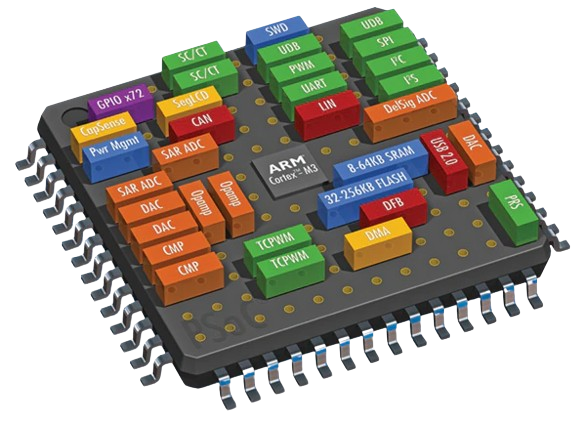
\includegraphics[width=1\linewidth]{resources/images/peripherals.png}
    \end{figure}
    \end{column}
    \begin{column}{0.5\textwidth}
    Periféricos comunes
    \noindent\rule{\textwidth}{0.5pt}
    \begin{itemize}
        \item General Purpose Input Output (GPIO)
        \item Analog to Digital Converter (ADC)
        \item Digital to Analog Converter (DAC)
        \item System Timer (Systick) y otros Timers
        \item Universal Synchronous Asynchronous Receiver Transmitter (USART)
        \item Inter-Integrated Circuit (I2C)
        \item Serial Peripherial Interface (SPI)
        \item Universal Serial Bus (USB)
    \end{itemize}
    \end{column}
\end{columns}
\end{frame}

\subsection{Matriz de conmutación}
\begin{frame}{Fundamentos de Programación para Sistemas Embebidos}{Matriz de conmutación}
\begin{columns}
\begin{column}{0.3\textwidth}
Cada pin tiene múltiples funciones asociadas. Se selecciona solo una de ellas de acuerdo a lo que se defina en la SWM y el IOCON.
\end{column}
\begin{column}{0.7\textwidth}
\begin{figure}
\centering
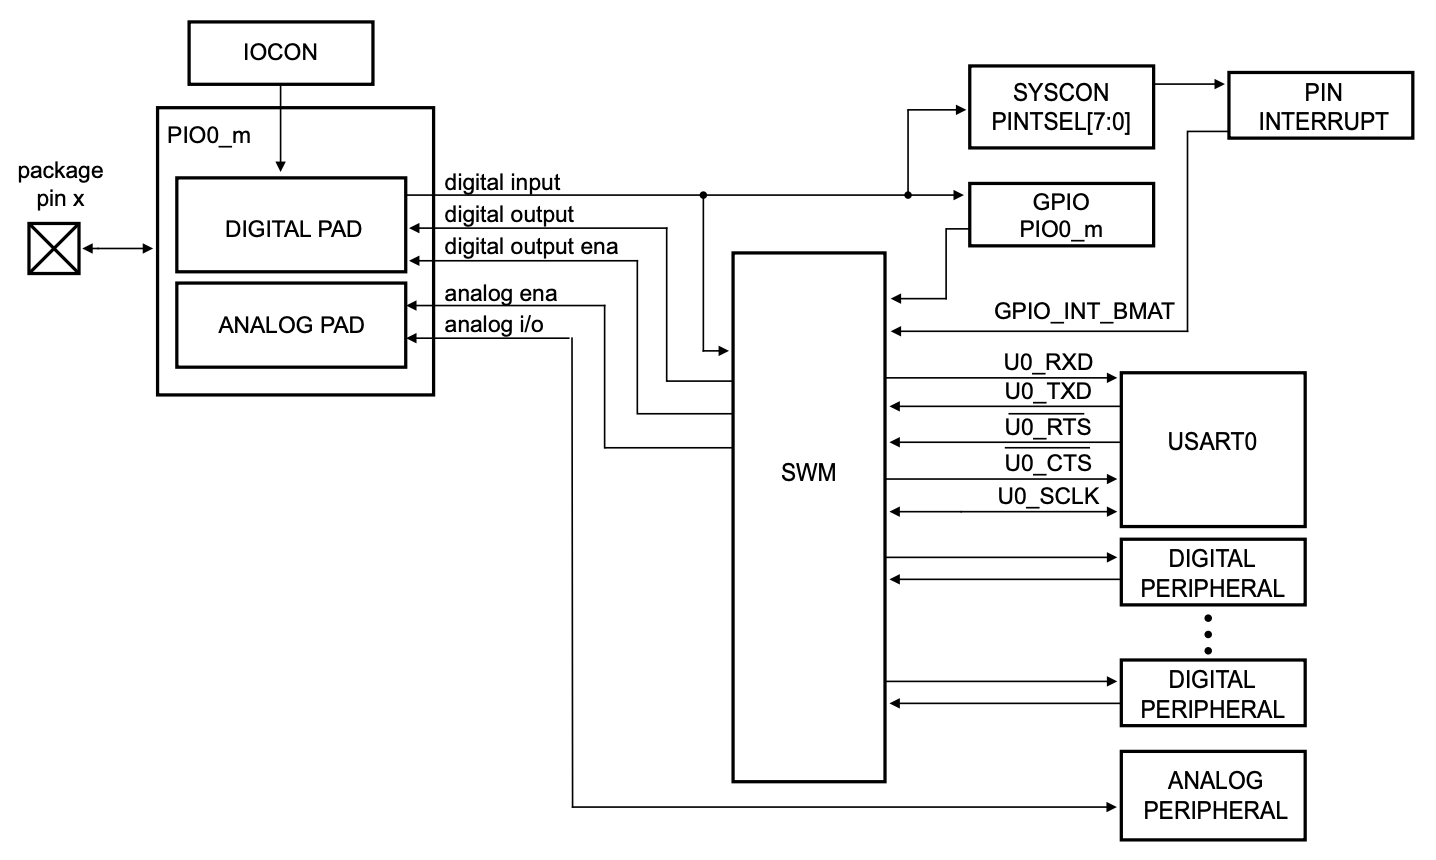
\includegraphics[width=0.75\linewidth]{resources/images/swm.png}
\end{figure}
\end{column}
\end{columns}
\end{frame}

\section{USART}
\subsection{Generalidades}
\begin{frame}{Fundamentos de Programación para Sistemas Embebidos}{Generalidades del USART}
\begin{itemize}
    \item Comunicación full-duplex.
    \item Puede trabajar en modo sincrónico o asincrónico.
    \item Paquetes de datos de 7, 8 o 9 bits.
    \item Baudrates estándares incluyen 4800, 9600, 19200, 38400, 57600, 115200.
    \item Los pines de RX y TX deben cruzarse entre dispositivos.
\end{itemize}
\begin{figure}
\centering
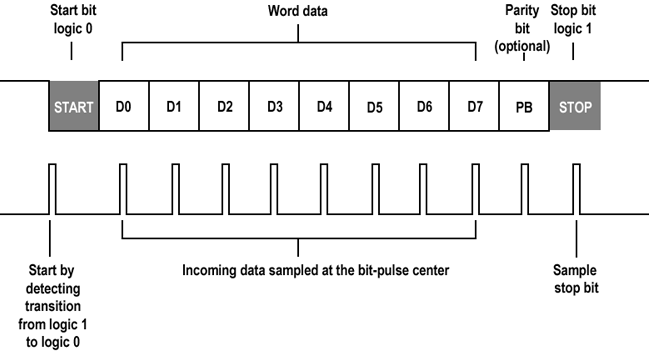
\includegraphics[width=0.45\linewidth]{resources/images/uart_frame.png}
\end{figure}
\end{frame}

\subsection{Asignación de pines}
\begin{frame}{Fundamentos de Programación para Sistemas Embebidos}{Asignación de pines del USART}
\begin{columns}
\begin{column}{0.5\textwidth}
\begin{itemize}
    \item Se usa \textcolor{myblue}{SWM\_SetMovablePinSelect} para elegir los pines que van a cumplir la función de USART.
    \item Se pasa primero el puntero a la matriz de conmutación (SWM), luego funcion que cumple (\textcolor{myblue}{swm\_select\_movable\_t}) y luego el puerto y pin (\textcolor{myblue}{swm\_port\_pin\_type\_t}).
    \item Se puede seleccionar estas funciones para prácticamente cualquier pin.
\end{itemize}
\end{column}
\begin{column}{0.5\textwidth}
\lstinputlisting[language=c, basicstyle=\tiny]{resources/listings/usart_swm.c}
\end{column}
\end{columns}
\end{frame}

\subsection{Inicialización}
\begin{frame}{Fundamentos de Programación para Sistemas Embebidos}{Inicialización del USART}
\begin{columns}
\begin{column}{0.6\textwidth}
\lstinputlisting[language=c, basicstyle=\tiny]{resources/listings/usart_init.c}
\end{column}
\begin{column}{0.4\textwidth}
\begin{itemize}
    \item Con \textcolor{myblue}{CLOCK\_Select} se elige la fuente de clock para el periférico.
    \item En la estructura del tipo \textcolor{myblue}{usart\_config\_t} se  configura: baudios, paridad, bits de stop, tamaño del paquete y la habilitación del RX y TX.
\end{itemize}
\end{column}
\end{columns}
\end{frame}

\subsection{Lectura y escritura}
\begin{frame}{Fundamentos de Programación para Sistemas Embebidos}{Lectura y escritura del USART}
\begin{columns}
\begin{column}{0.7\textwidth}
\begin{itemize}
    \item Se usa \textcolor{myblue}{USART\_WriteBlocking} para mandar un array o puntero a \textcolor{myblue}{uint8\_t}.
    \item El puntero debe ser casteado correctamente si el tipo de dato original era otro.
    \item Se debe indicar la cantidad de bytes que se quieren enviar por USART.
    \item Se usa \textcolor{myblue}{USART\_ReadBlocking} para leer una cantidad determinada de bytes del USART.
    \item Es necesario indicar un puntero a \textcolor{myblue}{uint8\_t} o array de ese tipo para determinar el destino de lo leído.
    \item Como el nombre lo indica, ambas funciones son bloqueantes.
\end{itemize}
\end{column}
\begin{column}{0.3\textwidth}
\lstinputlisting[language=c, basicstyle=\tiny]{resources/listings/usart_read_write.c}
\end{column}
\end{columns}
\end{frame}

\section{I2C}
\subsection{Generalidades}
\begin{frame}{Fundamentos de Programación para Sistemas Embebidos}{Generalidades del I2C}
\begin{itemize}
    \item Permite la conexión de múltiples dispositivos esclavos con solo un bus de datos (SDA) y clock (SCL).
    \item Cada dispositivo tiene una dirección única en el bus de 7 bits.
    \item Soporta velocidades estándares de 100Kb/s (Standard-mode), 400Kb/s (Fast-mode), 1Mb/s (Fast-mode Plus) y 3.4Mb/s (High-speed mode).
\end{itemize}
\begin{figure}
\centering
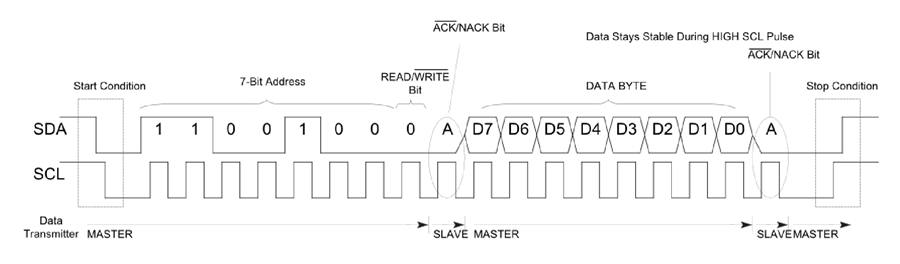
\includegraphics[width=0.75\linewidth]{resources/images/i2c.png}
\end{figure}
\end{frame}

\begin{frame}{Fundamentos de Programación para Sistemas Embebidos}{Generalidades del I2C}
\begin{columns}
\begin{column}{0.5\textwidth}
\begin{figure}
    \centering
    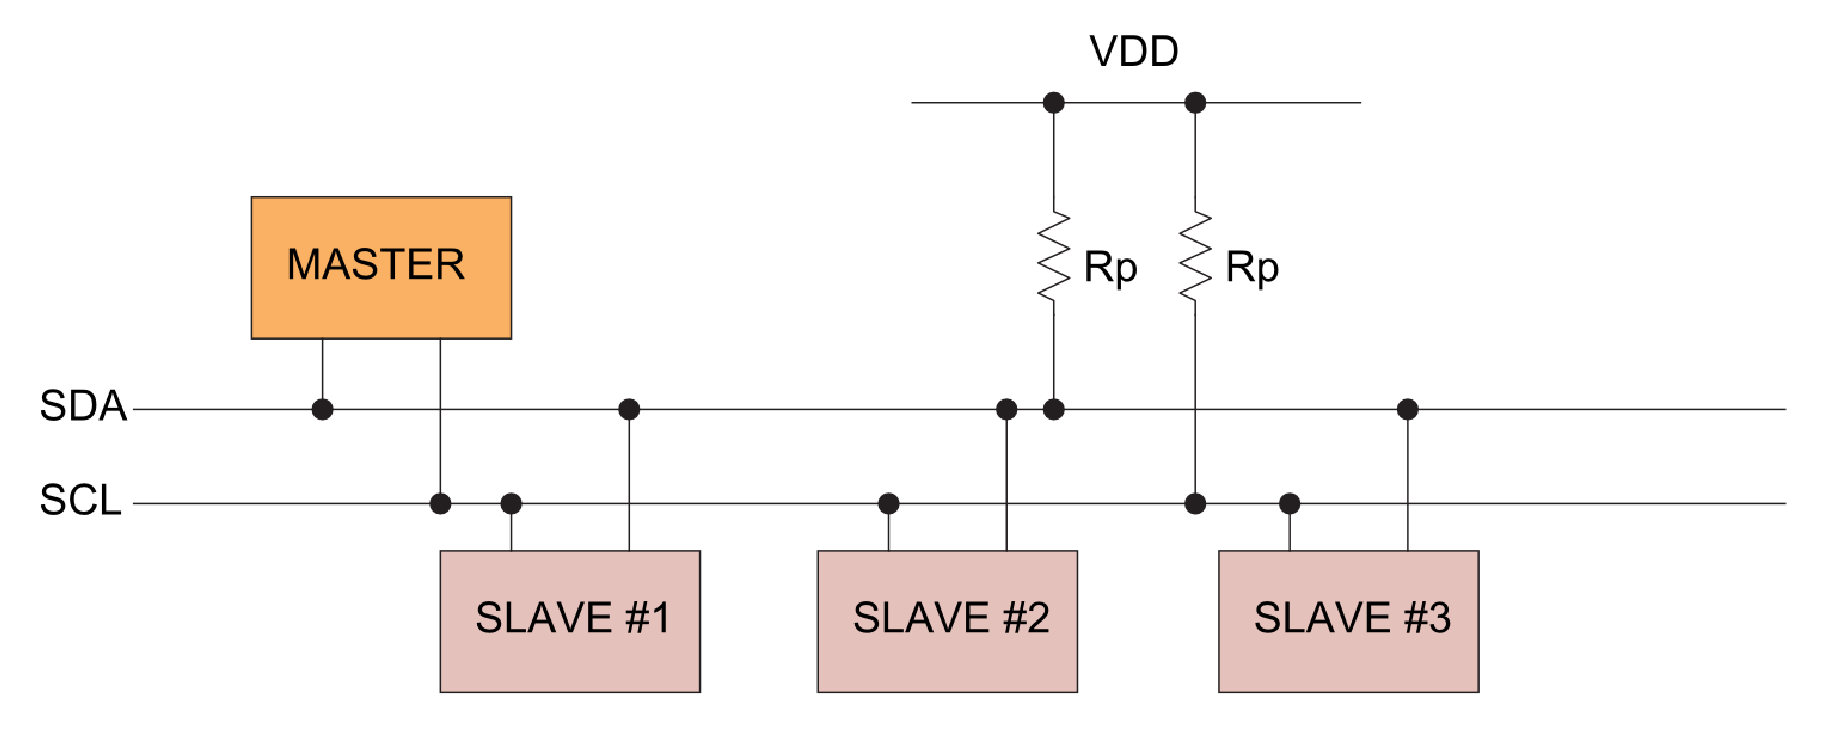
\includegraphics[width=1\linewidth]{resources/images/i2c_pullups.png}
\end{figure}
\end{column}
\begin{column}{0.5\textwidth}
\begin{itemize}
    \item Comunicación half-duplex.
    \item Para funcionar, el protocolo requiere resistencias de pull-up en SDA y SCL.
    \item Los pines asociados a I2C suelen ser salidas open-collector u open-drain.
    \item Las pull-ups ayudan que el estado por defecto del I2C sea high.
\end{itemize}
\end{column}
\end{columns}
\end{frame}

\subsection{Asignación de pines}
\begin{frame}{Fundamentos de Programación para Sistemas Embebidos}{Asignación de pines del I2C}
\begin{columns}
\begin{column}{0.5\textwidth}
\begin{itemize}
    \item Se usa \textcolor{myblue}{SWM\_SetMovablePinSelect} para elegir los pines que van a cumplir la función de I2C.
    \item En algunos microcontroladores, existen buses de I2C especialmente rápido que solo pueden usarse en pines fijos usando la función \textcolor{myblue}{SWM\_SetFixedPinSelect}.
    \item Exceptuando el caso anterior, cualquier pin suele poder usarse como SDA y SCL para el I2C.
\end{itemize}
\end{column}
\begin{column}{0.5\textwidth}
\lstinputlisting[language=c, basicstyle=\tiny]{resources/listings/i2c_pins.c}
\end{column}
\end{columns}
\end{frame}

\subsection{Inicialización}
\begin{frame}{Fundamentos de Programación para Sistemas Embebidos}{Inicialización del I2C}
\begin{columns}
\begin{column}{0.5\textwidth}
\lstinputlisting[language=c, basicstyle=\tiny]{resources/listings/i2c_init.c}
\end{column}
\begin{column}{0.5\textwidth}
\begin{itemize}
    \item Con \textcolor{myblue}{CLOCK\_Select} se elige la fuente de clock para el periférico.
    \item Con la estructura del tipo \textcolor{myblue}{i2c\_master\_config\_t} se puede configurar si el dispositivo va a funcionar como Master y la velocidad de clock para la comunicación siempre que sea posible generarla en ese pin.
\end{itemize}
\end{column}
\end{columns}
\end{frame}

\subsection{Escritura}
\begin{frame}{Fundamentos de Programación para Sistemas Embebidos}{Escritura por I2C}
\begin{columns}
\begin{column}{0.5\textwidth}
\begin{itemize}
    \item La función \textcolor{myblue}{I2C\_MasterStart} produce la condición de start en el bus.
    \item Para iniciar se pasa el bus usado, la dirección del esclavo y una constante del tipo \textcolor{myblue}{i2c\_direction\_t} para indicar si se escribe o se lee (\textcolor{myblue}{kI2C\_Write}).
    \item Para escribir, se usa \textcolor{myblue}{I2C\_MasterWriteBlocking}, pasando un array o puntero con los datos en formato \textcolor{myblue}{uint8\_t} y la cantidad de bytes a enviar.
    \item Se termina la comunicación con \textcolor{myblue}{I2C\_MasterStop}.
\end{itemize}
\end{column} 
\begin{column}{0.5\textwidth}
\lstinputlisting[language=c, basicstyle=\tiny]{resources/listings/i2c_write.c}
\end{column}
\end{columns}
\end{frame}

\subsection{Lectura}
\begin{frame}{Fundamentos de Programación para Sistemas Embebidos}{Lectura por I2C}
\begin{columns}
\begin{column}{0.5\textwidth}
\lstinputlisting[language=c, basicstyle=\tiny]{resources/listings/i2c_write.c}
\end{column} 
\begin{column}{0.5\textwidth}
\begin{itemize}
    \item La función \textcolor{myblue}{I2C\_MasterStart} inicia la comunicación.
    \item Se pasa a la función el valor de \textcolor{myblue}{kI2C\_Read} para iniciar una lectura.
    \item Para leer, se usa \textcolor{myblue}{I2C\_MasterReadBlocking}, pasando un array o puntero a \textcolor{myblue}{uint8\_t} donde guardar los datos y la cantidad de bytes a leer.
    \item Se termina la comunicación con \textcolor{myblue}{I2C\_MasterStop}.
\end{itemize}
\end{column}
\end{columns}
\end{frame}

\section{PWM}
\subsection{Generalidades}
\begin{frame}{Fundamentos de Programación para Sistemas Embebidos}{Generalidades del PWM}
\begin{itemize}
    \item Generan señales contínuas pulsantes de frecuencia fija y ancho de pulso variable.
    \item El efecto final es que la carga ve una señal de tensión media entre 0 y el valor de $V_{CC}$.
    \item Los valores de ancho de pulso suelen expresarse entre 0 y 1.
    \item Típicamente usado para controlar velocidad de motores, intensidades lumínicas, salidas analógicas y generación de senoidales.
\end{itemize}
\begin{figure}
\centering
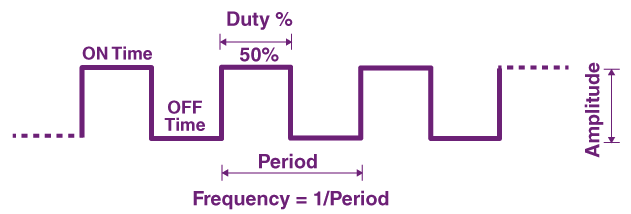
\includegraphics[width=0.5\linewidth]{resources/images/pwm.png}
\end{figure}
\end{frame}

\subsection{Asignación de pines}
\begin{frame}{Fundamentos de Programación para Sistemas Embebidos}{Asignación de pines para PWM}
\begin{columns}
\begin{column}{0.5\textwidth}
\begin{itemize}
    \item Se usa \textcolor{myblue}{SWM\_SetMovablePinSelect} para elegir el pin que va a generar una salida PWM.
    \item Los PWM se generan con Timers, en el caso del LPC845, el Timer por excelencia es el SCTimer.
    \item En el caso del LPC845, hay disponibles cuatro salidas para PWM.
\end{itemize}
\end{column}
\begin{column}{0.5\textwidth}
\lstinputlisting[language=c, basicstyle=\tiny]{resources/listings/pwm_swm.c}  
\end{column}
\end{columns}
\end{frame}

\subsection{Inicialización}
\begin{frame}{Fundamentos de Programación para Sistemas Embebidos}{Inicialización del PWM}
\begin{columns}
\begin{column}{0.5\textwidth}
\lstinputlisting[language=c, basicstyle=\tiny]{resources/listings/pwm_init_1.c}
\end{column}
\begin{column}{0.5\textwidth}
\begin{itemize}
    \item Se puede obtener una configuración por defecto con \textcolor{myblue}{SCTIMER\_GetDefaultConfig}.
    \item En la estructura del tipo \textcolor{myblue}{sctimer\_pwm\_signal\_param\_t} se pueden configurar cuál de las salidas del Timer se va a usar, la lógica y el porcentaje de ancho de pulso.
\end{itemize}
\end{column}
\end{columns}
\end{frame}

\begin{frame}{Fundamentos de Programación para Sistemas Embebidos}{Inicialización del PWM}
\begin{columns}
\begin{column}{0.5\textwidth}
\lstinputlisting[language=c, basicstyle=\tiny]{resources/listings/pwm_init_2.c}
\end{column}
\begin{column}{0.5\textwidth}
\begin{itemize}
    \item Con la función \textcolor{myblue}{SCTIMER\_SetupPWM} se puede configurar lo establecido en la estructura \textcolor{myblue}{sctimer\_pwm\_signal\_param\_t} y otros parámetros como la frecuencia del PWM y frecuencia de base del periférico.
    \item La función \textcolor{myblue}{SCTIMER\_StartTimer} es la encargada de dar inicio al Timer con la configuración establecida.
\end{itemize}
\end{column}
\end{columns}
\end{frame}

\subsection{Cambio de ciclo de trabajo}
\begin{frame}{Fundamentos de Programación para Sistemas Embebidos}{Cambio de ciclo de trabajo del PWM}
\begin{columns}
\begin{column}{0.5\textwidth}
\lstinputlisting[language=c, basicstyle=\tiny]{resources/listings/pwm_duty.c}
\end{column}
\begin{column}{0.5\textwidth}
\begin{itemize}
    \item La función \textcolor{myblue}{SCTIMER\_UpdatePwmDutycycle} es la que actualiza el ancho de pulso del PWM, requiere la salida que se quiere modificar, el ancho de pulso y el evento registrado anteriormente.
    \item El valor de ancho de pulso se especifica en 0 a 100.
    \item Se especifica la salida del SCTimer, no el pin mapeado a la salida.
\end{itemize}
\end{column}
\end{columns}
\end{frame}

% \section{SPI}
% \subsection{Generalidades}
% \begin{frame}{Fundamentos de Programación para Sistemas Embebidos}{Generalidades del SPI}
% \begin{columns}
% \begin{column}{0.5\textwidth}
% \begin{itemize}
%     \item Comunicación serial full-duplex.
%     \item Tiene un bus de datos de master a slave (MOSI) y otro separado para slave a master (MISO).
%     \item Soporta múltiples dispositivos conectados al mismo bus.
%     \item Para determinar qué dos dispositivos se comunican, se usa una linea de CS (Chip Select) para cada dispositivo que se activa con nivel bajo.
% \end{itemize}
% \end{column}
% \begin{column}{0.5\textwidth}
% \begin{figure}
% \centering
% 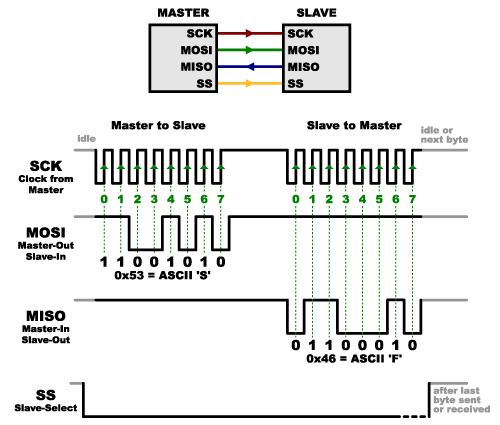
\includegraphics[width=0.75\linewidth]{resources/images/spi.png}
% \end{figure}    
% \end{column}
% \end{columns}
% \end{frame}

% \subsection{Asignación de pines}
% \begin{frame}{Fundamentos de Programación para Sistemas Embebidos}{Asignación de pines del SPI}
% \begin{columns}
% \begin{column}{0.5\textwidth}
% \lstinputlisting[language=c, basicstyle=\tiny]{resources/listings/spi_swm.c}
% \end{column}
% \begin{column}{0.5\textwidth}
% \begin{itemize}
%     \item 
% \end{itemize}
% \end{column}
% \end{columns}
% \end{frame}

\section{Ejercicios}
\begin{frame}{Fundamentos de Programación para Sistemas Embebidos}{Ejercicios}
    Algunas propuestas para practicar
    \noindent\rule{\textwidth}{0.75pt}
    \begin{enumerate}
        \item En un proyecto llamado \textbf{03\_light\_control}, hacer un programa que lea la intensidad lumínica indicada por el BH1750 y aumentar el brillo del LED D1 hasta alcanzar un maximo cuando la intensidad lumínica es mínima y un brillo mínimo cuando esta es máxima.
        \item En un proyecto llamado \textbf{03\_pwm\_sine\_wave}, generar una señal de PWM apropiada para lograr, con un filtro pasa banda, una senoidal de 10KHz.
        \item En un proyecto llamado \textbf{03\_servo\_control}, una señal de PWM apropiada para cubrir el ángulo de giro completo de un servomotor SG90 controlado por la indicación del potenciómetro R22.
    \end{enumerate}
    \noindent\rule{\textwidth}{0.75pt}
    Cada ejercicio que se resuelva, subirlo al repositorio personal del curso.
\end{frame}

\section{Referencias}
\begin{frame}{Fundamentos de Programación para Sistemas Embebidos}{Referencias}
    Algunos recursos útiles
    \noindent\rule{\textwidth}{0.75pt}
    \begin{multicols}{2}
    \begin{itemize}
        \item \href{https://github.com/utn-fra-lse/lpc845/blob/main/docs/UM11029.pdf}{Manual del LPC845}
        \item \href{https://github.com/utn-fra-lse/lpc845/blob/main/docs/UM11181.pdf}{Manual del LPC845 Breakout Board}
        \item \href{https://mcuxpresso.nxp.com/api_doc/dev/116/modules.html}{Documentación del SDK del LPC845}
        \item \href{https://github.com/utn-fra-lse/lpc845/blob/main/docs/BASE_KIT_V0.pdf}{Esquemático del kit del laboratorio}
        \item \href{https://www.cbtnuggets.com/blog/communication/half-duplex-vs-full-duplex}{Half-Duplex vs Full-Duplex}
        \item \href{https://www.nxp.com/docs/en/user-guide/UM10204.pdf}{I2C-bus specification and user manual}
        \item \href{https://www.ti.com/lit/an/sbaa565/sbaa565.pdf?ts=1722944333411}{A Basic Guide to I2C}
        \item \href{https://www.mouser.com/datasheet/2/348/bh1750fvi-e-186247.pdf?srsltid=AfmBOorrR8jrAGXGPYKRRWE16YcldiiGN0-D3jy5KHvUM9A1WPh_ohTP}{Hoja de datos del BH1750}
        \item \href{http://www.ee.ic.ac.uk/pcheung/teaching/DE1_EE/stores/sg90_datasheet.pdf}{Hoja de datos de servo motor SG90}
    \end{itemize}
    \end{multicols}
\end{frame}

\end{document}
